\PassOptionsToPackage{utf8}{inputenc}
\documentclass{bioinfo}
\copyrightyear{2015} \pubyear{2015}

\access{Advance Access Publication Date: Day Month Year}
\appnotes{Manuscript Category}



%%% PACKAGES

\usepackage{xr}
\externaldocument{supplement}


\usepackage{booktabs} % for much better looking tables
\usepackage{array} % for better arrays (eg matrices) in maths
% \usepackage{paralist} % very flexible & customisable lists (eg. enumerate/itemize, etc.)
%   \let\itemize\compactitem
%   \let\enditemize\endcompactitem
%   \let\enumerate\compactenum
%   \let\endenumerate\endcompactenum
%   \let\description\compactdesc
%   \let\enddescription\endcompactdesc
%   \pltopsep=1pt
%   \plitemsep=1pt
%   \plparsep=1pt
\usepackage{hyperref}
\usepackage{xspace}
%\usepackage{geometry}
\usepackage{amsmath,amssymb}
\usepackage{bm}
\usepackage{verbatim}
\usepackage{longtable}
\usepackage[vlined]{algorithm2e}

\usepackage{inconsolata}

\usepackage{xifthen}
\usepackage{stmaryrd}

\usepackage{xcolor}

\usepackage{todonotes}


\hypersetup{
    bookmarks=false,         % show bookmarks bar?
    unicode=false,          % non-Latin characters in Acrobat’s bookmarks
    pdftoolbar=true,        % show Acrobat’s toolbar?
    pdfmenubar=true,        % show Acrobat’s menu?
    pdffitwindow=true,     % window fit to page when opened
    pdfstartview={FitH},    % fits the width of the page to the window
    colorlinks=true,       % false: boxed links; true: colored links
%    linkcolor=red!70!black,          % color of internal links (change box color with linkbordercolor)
%    citecolor=red!70!black,        % color of links to bibliography
    linkcolor=black,          % color of internal links (change box color with linkbordercolor)
    citecolor=black,        % color of links to bibliography
    filecolor=magenta,      % color of file links
    urlcolor=red!70!black           % color of external links
}

%%%%%%%%%%%%%%%%%%%%%%%%%%%%%%%%%%%%%%%%
%% Rolf's includegraphicstop
\makeatletter
\newsavebox{\@alignepsbox}
\newlength{\@aligneps}
\newcommand{\includegraphicstop}[2][]{%
\sbox{\@alignepsbox}{\includegraphics[#1]{#2}}%
\setlength{\@aligneps}{-\ht\@alignepsbox}%
\addtolength{\@aligneps}{2ex}%
\raisebox{\@aligneps}{\usebox{\@alignepsbox}}}
\makeatother


%\makeatletter
%\let\oldlt\longtable
%\let\endoldlt\endlongtable
%\def\longtable{\@ifnextchar[\longtable@i \longtable@ii}
%\def\longtable@i[#1]{\begin{figure}[t]
%\onecolumn
%\begin{minipage}{0.5\textwidth}
%\oldlt[#1]
%}
%\def\longtable@ii{\begin{figure}[t]
%\onecolumn
%\begin{minipage}{0.5\textwidth}
%\oldlt
%}
%\def\endlongtable{\endoldlt
%\end{minipage}
%\twocolumn
%\end{figure}}
%\makeatother

%%%%%%%%%%%%%%%%% Theorems %%%%%%%%%%%%%%%%%%%%%%%%%

 \newtheorem{theorem}{Theorem}
 \newtheorem{definition}[theorem]{Definition}
 \newtheorem{remark}[theorem]{Remark}
 \newtheorem{corollary}[theorem]{Corollary}
 \newtheorem{lemma}[theorem]{Lemma}
 \newtheorem{proposition}[theorem]{Proposition}

\newtheorem{observation}[theorem]{Observation}

%\newtheorem{algorithm}{Algorithm}
\newtheorem{axiom}{Axiom}
\newtheorem{hypothesis}{Working Hypothesis}
\renewenvironment{proof}[1][]{\noindent \em Proof\ifthenelse{\equal{#1}{}}{}{ (#1)}:~}{}

%%% macros for notation in DP framework
\newcommand{\network}{\mathcal{N}}
\newcommand{\val}{\bar S} % valuation aka assignment
\newcommand{\dep}{\operatorname{dep}}
\newcommand{\energy}[1]{\operatorname{e}_{#1}}
\newcommand{\numberof}{\operatorname{\#}}
\newcommand{\partfun}[1]{Z_{#1}}
\newcommand{\separator}[2]{\operatorname{sep}(#1,#2)}
\newcommand{\difference}[2]{\operatorname{diff}(#1 \rightarrow #2)}
\newcommand{\real}{\mathbb{R}}
\newcommand{\genmarg}[1]{(\!|\!#1\!|\!)}
\newcommand{\gencomb}[1]{\langle\!|#1|\!\rangle}
\newcommand{\Message}[2]{m_{#1\rightarrow #2}}


\newcommand{\energyModel}{{\cal M}}
\newcommand{\structureElements}{{\cal SE}}
\newcommand{\powerSet}[1]{2^{#1}}
\newcommand{\underConstruction}[1]{{\LARGE$\triangle$\Large\!\!\!\!!}$\quad$\textcolor{red}{#1}}
\newcommand{\argmin}{\operatorname*{arg\,min}}
\newcommand{\objective}{{\mathbb{F}}}

\newcommand{\partseqs}{\mathcal{P\!S}}
\newcommand{\B}{\mathcal{B}}
\newcommand{\F}{\mathcal{F}}
\newcommand{\I}{\mathcal{I}}
\newcommand{\R}{\mathcal{R}}
\renewcommand{\S}{\mathcal{S}}
\newcommand{\X}{\mathcal{X}}
\newcommand{\Y}{\mathcal{Y}}

\newcommand{\width}{w}

\newcommand{\sample}{\texttt{Sample}}
\newcommand{\elim}[2]{\operatorname{elim}(#1,#2)}
\newcommand{\edgesToR}{E^r_T}

\newcommand{\phitotal}{\phi_{\operatorname{m}}}

\newcommand{\Ebp}[2]{E^{\textrm{bp}}_{#1}(#2)}
\newcommand{\Ehp}[1]{E^{\textrm{hp}}(#1)}
\newcommand{\Eint}[1]{E^{\textrm{int}}(#1)}

\newcommand{\Def}[1]{{\bfseries #1}}

\newcommand{\TargetE}{E^{\star}}

\newcommand{\TODO}[1]{\textcolor{red!70!black}{\textbf{TODO: #1}}}

\newcommand{\parHead}[1]{\Final{\paragraph{#1}}}

\newcommand{\Final}[1]{\begingroup\color{red!70!black}#1\endgroup}
%% Uncomment the line below for ``Final'' version
%\renewcommand{\Final}[1]{}

\newcommand{\Design}[1]{{\sf Designs}^{\star}(#1)}
\newcommand{\NumDesign}{\ensuremath{\#}{\sf Designs}\xspace}
\newcommand{\IS}[1]{{\sf IndSets}(#1)}
\newcommand{\Nuc}[1]{{\sf #1}}
\newcommand{\Ab}{\Nuc{A}}
\newcommand{\Cb}{\Nuc{C}}
\newcommand{\Gb}{\Nuc{G}}
\newcommand{\Ub}{\Nuc{U}}

\newcommand{\GCb}{\Gb\Cb}

\newcommand{\Software}[1]{{\ttfamily #1}}

\newcommand{\evalfor}[2]{#1\llbracket{}#2\rrbracket{}}
\newcommand{\substitute}[2]{#1\!\oplus\!#2}

\renewcommand{\gets}{:=}

\setlength{\parskip}{.2em}

\newcommand{\RNAblueprint}{{\tt \bfseries{}\color{black!75} RNA\textcolor{blue!70!black}{Blue}Print}}
\newcommand{\ourprog}{{\tt \bfseries{}\color{black!75}RNA\textcolor{red!70!black}{Red}Print}}

\newcommand{\Energy}[2]{E(#2;#1)}

\newcommand{\EnergyTurner}{E_{\text{T}}}
\newcommand{\EnergyStacking}{E_{\text{st}}}

%%% end macro defs



\begin{document}
\firstpage{1}

\subtitle{Research Article}

\title[Efficient Sampling for Multi-Target RNA Design]{Fixed-Parameter Tractable Sampling for RNA Design with Multiple Target Structures}
\author[Hammer, Ponty, Wang and Will]{Stefan Hammer\,$^{\text{\sfb 1,2,3}}$, Yann Ponty\,$^{\text{\sfb 4,5,}\star}$, Wei Wang\,$^{\text{\sfb 4}}$ and Sebastian Will\,$^{\text{\sfb 2}}$}
\address{$^{\text{\sf 1}}$University Leipzig, Department of Computer Science and Interdisciplinary Center for Bioinformatics, 04107 Leipzig, Germany;
$^{\text{\sf 2}}$University of Vienna, Faculty of Chemistry, Department of Theoretical Chemistry, 1090 Vienna, Austria;
$^{\text{\sf 3}}$University of Vienna, Faculty of Computer Science, Research Group Bioinformatics and
Computational Biology, 1090 Vienna, Austria;
$^{\text{\sf 4}}$CNRS UMR 7161 LIX, Ecole Polytechnique, Bat. Turing, 91120 Palaiseau, France;
and $^{\text{\sf 5}}$ AMIBio team, Inria Saclay, Bat Alan Turing, 91120 Palaiseau, France}

\corresp{$^\ast$To whom correspondence should be addressed.}

\history{Received on XXXXX; revised on XXXXX; accepted on XXXXX}

\editor{Associate Editor: XXXXXXX}

\abstract{\textbf{Motivation:} The design of multi-stable RNA molecules has important applications in biology, medicine, and biotechnology. Synthetic design approaches profit strongly from effective in-silico methods, which can tremendously impact their cost and feasibility. \\
  \textbf{Results:} We revisit a central ingredient of most in-silico
  design methods: the sampling of sequences for the design of
  multi-target structures, possibly including pseudoknots. For this
  task, we present the efficient, tree decomposition-based algorithm
  \ourprog{}. Our fixed parameter tractable approach is underpinned by
  establishing the $\#${\sf P}-hardness of uniform sampling. Modeling
  the problem as a constraint network, \ourprog{} supports generic
  Boltzmann-weighted sampling for arbitrary additive RNA energy
  models; this enables the generation of RNA sequences meeting
  specific goals like expected free energies or \GCb-content. Finally,
  we empirically study general properties of the approach and generate
  biologically relevant multi-target Boltzmann-weighted designs for a
  common design benchmark. Generating seed sequences with \ourprog{}, we demonstrate significant improvements over the previously best multi-target sampling strategy (uniform sampling).\\
  \textbf{Availability:} Our software is freely available at: \url{https://github.com/yannponty/RNARedPrint}\\
  \textbf{Contact:} \href{yann.ponty@lix.polytechnique.fr}{yann.ponty@lix.polytechnique.fr}\\
  \textbf{Supplementary information:} Supplementary data are available
  at \textit{Bioinformatics} online.}

\maketitle



\section{Introduction}
\parHead{Design, applications and motivation for multiple design.}Synthetic biology endeavors the engineering of artificial biological
systems, promising broad applications in biology, biotechnology and
medicine. Centrally, this requires the design of biological
macromolecules with highly specific properties and programmable functions.
In particular, RNAs present themselves as well-suited tools for
rational design targeting specific functions~\citep{Kushwaha2016}. RNA function is tightly
coupled to the formation of secondary structure, as well as changes in
base pairing propensities and the accessibility of regions, e.g. by
burying or exposing interaction sites~\citep{Rodrigo2014}. At the same time, the
thermodynamics of RNA secondary structure is well understood and its prediction is
computationally tractable~\citep{McCaskill1990}. Thus,  structure can serve as effective
proxy within rational design approaches, ultimately targeting catalytic~\citep{Zhang2013} or regulatory~\citep{Rodrigo2014} functions.

\parHead{Motivating multiple RNA design.} The function of many RNAs
depends on their selective folding into one or several alternative
conformations. Classic examples include riboswitches, which
notoriously adopt different stable structures upon binding a specific
ligand. Riboswitches have been a popular application of rational
design~\citep{Wachsmuth2013,Domin2017}, partly motivated by their
capacity to act as biosensors~\citep{Findeiss2017}. At the
co-transcriptional level, certain RNA families feature alternative,
evolutionarily conserved, transient structures~\citep{Zhu2013}, which
facilitate the ultimate adoption of functional structures at full
elongation.  More generally, simultaneous compatibility to multiple
structures is a relevant design objective for engineering kinetically
controlled RNAs, finally targeting prescribed folding pathways. Thus,
modern applications of RNA design often target multiple structures,
additionally aiming at other features, such as specific
\GCb-content (\GCb\%) as previously done by~\citet{Reinharz2013} or the presence/absence of
functionally relevant motifs (either anywhere or at specific
positions)~\citep{Zhou2013}; these objectives motivate flexible
computational design methods.

\parHead{On the importance of sampling for design.}
Many computational methods for RNA design rely on similar overall
strategies: initially generating one or several \Def{seed} sequences
and optimizing them subsequently. In many cases, the seed quality was
found to be critical for the empirical performance of RNA design
methods~\citep{Levin2012}. For instance, random seed generation
improves the prospect of subsequent optimizations, helping to overcome
local optima of the objective function, and increases the diversity
across designs~\citep{Reinharz2013}.  For single-target approaches,
\Software{INFO-RNA}~\citep{Busch2006} made significant improvements
mainly by starting its local search from the minimum energy sequence
for the target structure instead of (uniform) random sequences for the
early \Software{RNAinverse} algorithm~\citep{Hofacker1994}. This
strategy was later shown to result in unrealistically high
\GCb\% in designed sequences. To address this issue,
\Software{IncaRNAtion}~\citep{Reinharz2013} controls \GCb\%
through an adaptive sampling strategy.

\parHead{Specificities and similarities of multi-target design.}
Specifically, for multi-target design, virtually all available methods~\citep{Lyngsoe2012,HoenerzuSiederdissen2013,Taneda2015,Hammer2017} follow the same overall generation/optimization scheme.
%
Facing the complex sequence constraints induced by multiple targets, early methods such as \Software{Frnakenstein}~\citep{Lyngsoe2012} and \Software{Modena}~\citep{Taneda2015} did not attempt to solve sequence generation systematically, but rely on \emph{ad-hoc} sampling strategies.
%
Recently, the \Software{RNAdesign}
approach~\citep{HoenerzuSiederdissen2013}, coupled with powerful local
search within \RNAblueprint{}~\citep{Hammer2017}, solved the
problem of sampling seeds from the uniform distribution for multiple
targets. These methods adopt a graph coloring perspective, initially
decomposing the graph hierarchically using various decomposition
algorithms, and \Def{precomputing} the number of valid sequences
within each subgraph. The decomposition is then reinterpreted as a
decision tree to perform a \Def{stochastic backtrack}, inspired by
Ding and Lawrence~\citep{Ding2003}. Uniform sampling is achieved by
choosing individual nucleotide assignments with probabilities derived
from the subsolution counts. The overall complexity of
\Software{RNAdesign} grows like $\Theta(4^{\gamma})$, where the
parameter $\gamma$ is bounded by the length of the designed RNA;
typically, the decomposition strategy achieves much lower $\gamma$.

\parHead{Motivation.} The exponential time and space requirements of the \Software{RNAdesign} method already raise the question of the \Def{complexity of (uniform) sampling for multi-target design}. Since stochastic backtrack can be performed in linear time per sample, the method is dominated by the precomputation step, which requires counting valid designs. Thus, we focus on the question: \emph{Is there a polynomial-time algorithm to count valid multi-target designs?} In Section~\ref{sec:counting}, we answer in the negative, showing that there exists no such algorithm unless ${\sf P}={\sf NP}$. Our result relies on a surprising bijection (up to a trivial symmetry) between valid sequences  and independent sets of a bipartite graph, being the object of recent breakthroughs in approximate counting complexity~\citep{Bulatov2013,Cai2016}.
The hardness of counting (and conjectured hardness of sampling) does not preclude, however, practically applicable algorithms for counting and sampling. In particular, we wish to extend the flexibility of multi-structure design, leading to the following questions: \emph{How to sample, generally, from a Boltzmann distribution based on expressive energy models? How to enforce additional constraints, such as \GCb\%, complex sequence constraints, or the energy of individual structures?}


\begin{figure*}[t]
\begin{center}
    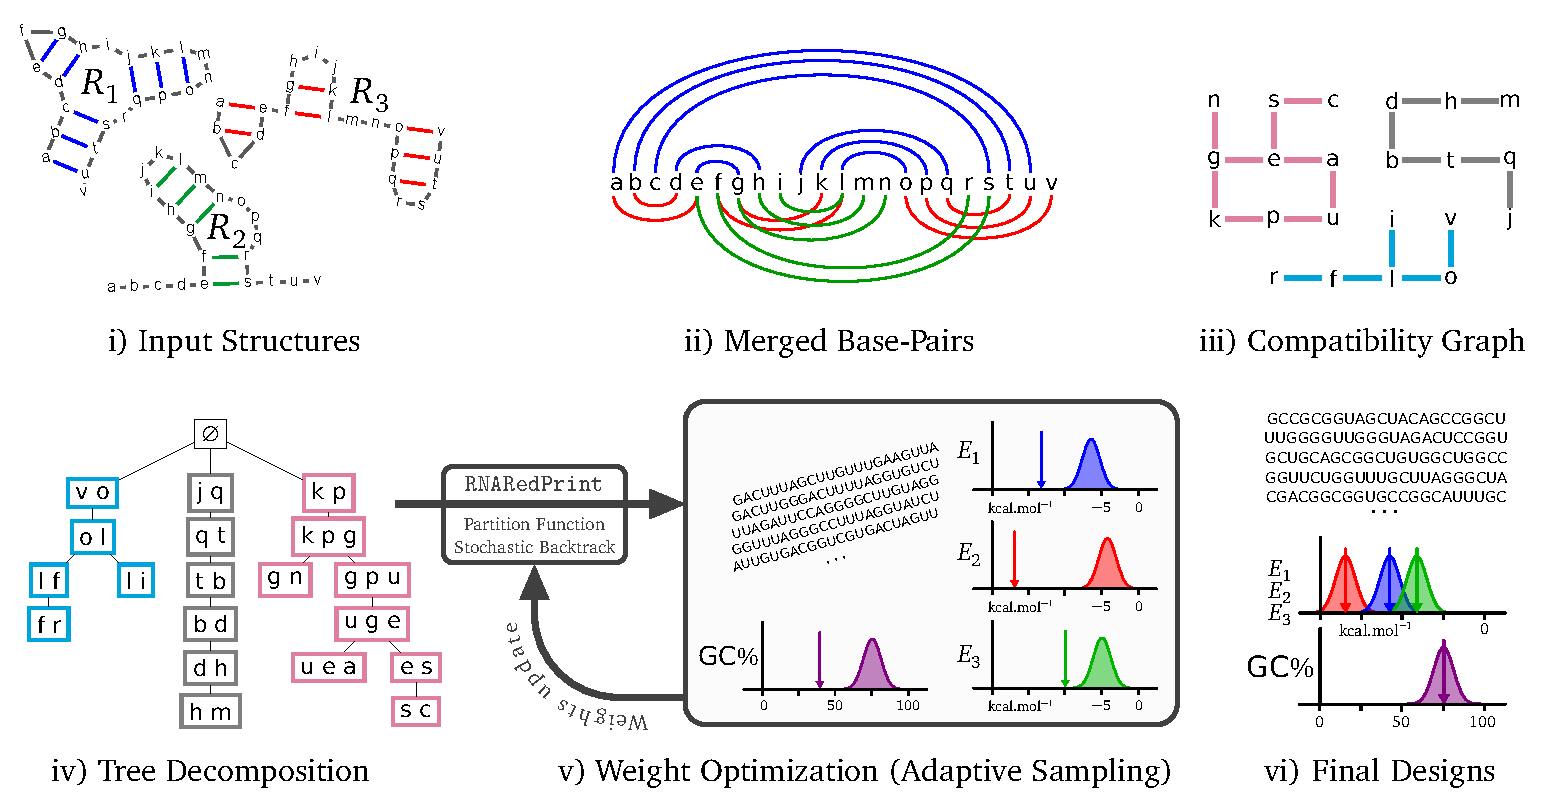
\includegraphics[width=.8\textwidth]{Workflow.pdf}
\end{center}
\caption{General outline of \ourprog{} for base pair-based energy models. From a set of target secondary structures (i), base-pairs are merged (ii) into a (base pair) dependency graph (iii) and transformed into a tree decomposition (iv). The tree is then used to compute the partition function, followed by a Boltzmann sampling of valid sequences (v). An adaptive scheme learns weights to achieve targeted energies and \GCb\%, leading to the production of suitable designs (vi).}
\label{fig:workflow}
\end{figure*}

To answer these questions, we introduce a generic framework (illustrated in~Fig.~\ref{fig:workflow}) enabling efficient Boltzmann-weighted sampling over RNA sequences with multiple target structures (Section~\ref{sec:FPT}). Guided by a \Def{tree decomposition} of the network, we devise dynamic programming to compute partition functions and sample sequences from the Boltzmann distribution%
% (Subsection~\ref{sec:PF})
. We show that these algorithms are \Def{fixed-parameter tractable} for the \Def{treewidth}%
% Subsection~\ref{sec:complexity}
%
; in practice, we limit this parameter by using state-of-the-art tree decomposition algorithms.
%Uniform sampling is handled as a special case of Boltzmann sampling, where each valid sequence receives energy zero and---consequently---computing partition functions specializes to counting.
By evaluating (partial) sequences in a weighted constraint
network, we support arbitrary multi-ary constraints and thus
arbitrarily complex energy models,
notably subsuming all commonly
used RNA energy models%
%(Subsection~\ref{sec:energy_models})
.  Moreover, we describe an \Def{adaptive
  sampling} strategy to control the free energies of the individual
target structures and \GCb\%%
% (SubSection~\ref{sec:multiBoltzmann})
. %
We observe that sampling based on less complex RNA energy models
(taking only the most important energy contributions into account)
still allows targeting realistic RNA energies in the well-accepted
Turner RNA energy model. The resulting combination of efficiency and
high accuracy finally enables generating biologically relevant
multi-target designs in our final application of our overall strategy
to a large set of multi-target RNA design instances from a
representative benchmark Section~\ref{sec:results}).

%In this work, we present a generic approach to multi-target sequence sampling that enables Boltzmann-weighted sampling (subsuming uniform sampling) for a wide class of objective functions that can even make use of the commonly used ``full-featured'' RNA energy models (like the Turner model~\citep{turner}). Due to its high expressivity the same framework allows combining objective functions with various hard and soft constraints, which can accommodate various desirable multi-target design scenarios.

%To provide a simple concrete example of multi-target design, consider designing a single sequence where all target structures are as stable as possible.
%That is, one asks for the sequence $S$ that minimizes the energy differences of the target structures to the minimum energy for this sequence among all possible structures; one aims to minimize
%   \begin{equation}
%\label{eq:design-objective}
%\sum_{\ell\in[1,k]} E(S;R_\ell) - E_0(S),
%\end{equation}
%over all sequences $S$, where $E_0(S):=\min_R E(S;R)$.
%
%The proposed Boltzmann-weighted sampling approach can support this design procedure by sampling start structures from the Boltzmann distribution over
%\begin{equation}
%\label{eq:sampling-objective} \sum_{\ell\in[1,k]} w_\ell E(S;R_\ell)
%\end{equation}
%or extensions thereof, e.g.~for controlling base frequencies. Suitable weights $w_\ell$ to accommodate the design objective can be approximated automatically after the machinery for Boltzmann sampling over such functions is set up.
%
%\TODO{Rewrite (from here to "Contributions"): sounds too negative}
%Notably, by Eq.~(\ref{eq:sampling-objective}) we do not suggest to sample over the energy difference of Eq.~$(\ref{eq:design-objective})$. The term $\min_R E(S;R)$, which---for each sequence---minimizes over the entire structure space, precludes efficient sampling even by the proposed approach.
%
%Already sampling over Eq.~(\ref{eq:sampling-objective}) strictly extends the only previously existing approach to controlled sampling from single to multi-target sampling (in complete analogy to IncaRNAtion only after GC content is controlled, which we present later) and subsumes uniform sampling for multi-target design.
%
%Naturally, also more complex objective functions are desirable for RNA design and have been discussed in the literature; e.g. the ensemble defect~\citep{Zadeh:2010}. Typically, more complex objective functions make design computationally much more challenging. Similarily, also the proposed sampling framework supports only a limited class of objective functions directly and efficiently---namely ``only'' all additive energy functions. Nevertheless, one can safely assume that the design under various more realistic objective functions profits from controlled sampling as long as the sampling is directed towards the final objective function.



%\TODO{Recycled material: To be merged with intro later}
%{\it
%This graph coloring perspective was the basis for the uniform sampling method of \Software{RNADesign} / \Software{RNAblueprint}, which decomposes the graph hierarchically, counts the solutions in subgraphs, and finally samples solutions. Essentially, an \Def{ear decomposition} is used as a decision tree, where decisions are made according to the subsolution counts in order to guarantee uniform sampling.
%
%However, highly desirable objectives of RNA design, such as a control over the energy of individual structures, require one to depart from the uniform generation, and therefore generalize this setting. First, instead of subsolution counts, one needs partition functions for guiding the sampling procedure. Second, in the case of realistic energy models %like Eq.~(\ref{eq:sampling-objective}) are based on realistic RNA energy models
%(e.g.~the Turner model), the atomic energy contributions depend on bases at more than two sequence positions---i.e. they cannot be captured by a strategy that only accounts for base-pairs.
%%
%
%
%These considerations motivate our sampling strategy, where we:
%\begin{itemize}
%\item Model RNA sequences as assignments over a constraint network. The network consists of one position per sequence position; constraints and energy contributions are modeled as functions of arbitrary arity over the positions, such that the total energy is the sum of all function values;
%\item Translate the dependency hyper-graph into a binary dependency graph by inserting cliques (Appendix), such that a tree decomposition with small treewidth can be computed by a generic tree decomposition algorithm;
%\item Compute the partition functions by specializing the generic ``Cluster Tree Elimination'' (CTE) dynamic programming algorithm, based on the cluster tree decomposition induced by the constraint network;
%
%\item Sample sequences are from the Boltzmann-distribution guided by the decomposition tree and the sub-partition functions.
%\end{itemize}
%}


\section{Definitions and problem statement}
\label{sec:problem-statement}

An \Def{RNA sequence $S$} is a word over the \Def{nucleotides
  alphabet} $\Sigma=\{\Ab,\Cb,\Gb,\Ub\}$; let $\S_n$ denote the set of
sequences of length $n$. An \Def{RNA (secondary) structure $R$ of
  length $n$} is a set of \Def{base pairs} $(i,j)$, where
$1\leq i<j\leq n$, where for all different $(i,j), (i',j')\in R$:
$\{i,j\}\cap\{i',j'\}=\emptyset$ (``degree $\leq$ 1'').
%
% We call an RNA structure $R$ \Def{non-crossing}, iff it does not
% contain any two different base pairs $(i,j)$ and $(i',j')$ such that
% $i\leq i'\leq j \leq j'.$
%
\Def{Valid base pair} must pair bases from
$\B:=\left\{\{\Ab,\Ub\},\{\Gb,\Cb\},\{\Gb,\Ub\}\right\}.$
Consequently, $S$ is \Def{valid} for $R$, iff $\{S_i,S_j\}\in \B$ for
all $(i,j)\in R$.

We consider a fixed set of target RNA structures
$\R:=\{R_1, \dots, R_k\}$ for sequences of length $n$. $\R$ induces a
\Def{base pair dependency graph} $G_{\R}$ with nodes $\{1,\dots,n\}$
and edges $\bigcup_{\ell\in[1,k]} R_\ell$, which describe the minimal
dependencies present in all relevant settings due to the requirement
of canonical base pairing.

One can interpret the valid sequences for $\R$ as colorings of
$G_{\R}$ in a slightly modified graph coloring variant, where the
colors (from $\Sigma$) assigned to adjacent vertices of $G_{\R}$ must
constitute valid base pairs.
%
The \Def{energy} of a sequence $S$ is defined by an \Def{energy
  function} $E$---defined for set of structures $\R$ and mapping
sequences to $\mathbb{R}\cup\{\infty\}$---as
$\Energy{\R}{S} \in \mathbb{R}\cup\{\infty\}$. In our setting, the
energy $\Energy{\R}{S}$ is typically chosen as a linear combination of
the energies of the single RNA structures (in some RNA energy model
that defines $E(S,R) \in \mathbb{R}\cup\{\infty\}$ for each
sequence $S$ and structure
$R$), as well as sequence-dependent features like \GCb\%. Formally, we
will require that
$\Energy{\R}{S}$ can be expressed as sum over functions values, where
each function depends on the nucleotides at certain positions of
$S$ (see below). Furthermore note that
$\Energy{\R}{S}$ is finite iff
$S$ is valid for each structure $R_1,\dots,R_k$.

At the core of this work, we study the computation of partition
functions over sequences.\smallskip\\
\textbf{Central problem (Partition function over sequences).}
  Given an energy function $E$ and a set $\R$ of structures of length $n$, compute the
  partition function
  \begin{equation}
    \label{eq:mainproblem}
    \partfun{E,\R} = \sum_{S\in\S_n} \exp(-\beta \Energy{\R}{S}),
  \end{equation}
  where $\beta$ denotes the inverse pseudo-temperature, and $\S_n$ the set of sequences of length $n$.

%We solve the problem efficiently for any fixed parameter $w$, whose value reflects the intrinsic complexity of the structures and energy function $E_\R$.
%
  As we elaborate in subsequent sections, our approach relies on
  breaking down the energy function $\Energy{\R}{S}$ into additive
  components, each depending on only few sequence positions. Given
  $\R$, we express $\Energy{\R}{S}$ as the sum of energy contributions $f(S)$
  over a set $\F$ (of functions $f:\S_n\to\real$),
  s.t.~$\Energy{\R}{S}=\sum_{f\in\F} f(S)$. This captures realistic RNA
  energy models---including nearest neighbor models,
  e.g.~\citet{Turner2009}, and even pseudoknot models,
  e.g. \citet{Andronescu2010}, while bounding the dependencies to
  sequence positions introduced by each single $f$. Formally, define
  the \Def{dependencies} $\dep(f)$ of $f$ as the minimum set of sequence
  positions $\I\subseteq\{1,\dots,n\}$, where $f(S)=f(S')$ for all
  sequences $S$ and $S'$ that agree at the positions in $\I$.

  Each set $\F$ of functions (on sequences of length $n$) induces a
  \Def{dependency graph} on sequence positions, namely the hypergraph
  $G_\F=(\{1,\dots,n\} ,\{\dep(f)\mid f\in \F\})$.  Our algorithms
  will critically rely on a \Def{tree decomposition} of the dependency
  graph, which we define below.
\begin{definition}[Tree decomposition and width]
  \label{def:treedecomp}
  Let $G=(X, E)$ be a hypergraph. A \Def{tree decomposition} of $G$ is
  a pair $(T,\chi)$, where $T$ is an unrooted tree/forest, and (for
  each $v\in T$) $\chi(v)\subseteq X$ is a set of vertices assigned to
  the node tree $v\in T$, such that
\begin{enumerate}
\item each $x\in X$ occurs in at least one $\chi(v)$;
\item for all $x\in X$, $\{ v \mid x \in \chi(v) \}$ induces a connected subtree of $T$;
\item for all $e\in E$, there is a node $v\in T$, such that $e\subseteq\chi(v)$.
\end{enumerate}
The \Def{width} of a tree decomposition $(T,\chi)$ is defined as
$\width(T,\chi) = \min_{u\in T} |\chi(u)| - 1 $. The \Def{treewidth}
of $G$ is the smallest width of any tree decomposition of $G$.
\end{definition}


\section{An FPT algorithm for the partition function and sampling of Boltzmann-weighted designs}
\label{sec:FPT}

For our algorithmic description, we translate the concepts of
Section~\ref{sec:problem-statement} to the formalism of constraint networks, here
specialized as RNA design network. This allows us to base our
algorithm on the cluster tree elimination (CTE) of~\citet{Dechter2013}.
%
In the RNA design network, (partially determined) RNA sequences
replace the more general concept of (partial) assignments in
constraint networks. Partially determined RNA sequences, for short
\Def{partial sequences}, are words $\val$ over the alphabet
$\Sigma\cup\{?\}$ equivalently representing the set ${\mathcal S}(\val)$
of RNA sequences, where for positions $1\leq i\leq n$,
$\val_i\in\Sigma$ implies $S_i=\val_i$ for all $S\in{\mathcal
  S}(\val)$. The positions $1\leq i\leq n$, where $\val_i\in\Sigma$,
are called \Def{determined} by $\val$ and form its \Def{domain}.
%
Since the functions $f\in\F$ of Section~\ref{sec:problem-statement}
depend on only the subset $\dep(f)$ of sequence positions, one can
evaluate them for partial sequences $\val$ that determine (at least)
the nucleotides at all positions in $\dep(f)$. Thus for functions $f$
and partial sequences $\val$ that determine $\dep(f)$, we write
$\evalfor{f}{\val}$ to \Def{evaluate $f$ for $\val$}; i.e.{}
$\evalfor{f}{\val} := f(S),$ for any sequence
$S\in{\mathcal S}(\val)$.

\begin{definition}
An \Def{RNA design network} (for sequences of length $n$) is a tuple $\network=(\X,\F)$, where\vspace{-6pt}
\begin{itemize}
\item $\X$ is the set of sequence positions $1,\dots,n$
\item $\F$ is a set of \Def{functions} $f:\S_n\to\real$
\end{itemize}
\end{definition}

%
The \Def{energy $\energy{\network}(S)$ of a sequence} $S$ in a network
$\network$ is defined as sum of the values of all functions in
$f\in\F$ evaluated for $S$, i.e.
$\energy{\network}(S) := \sum_{f\in\F} \evalfor{f}{S}.$

The network energy $\energy{\network}(S)$ corresponds to the energy in
Eq.~$(\ref{eq:mainproblem}),$ where this energy is modeled as sum of
the functions in $\F$. Consequently, $\partfun{\R}$ of
Eq.~$(\ref{eq:mainproblem})$ is modeled as network partition function
$\partfun{\network} := \sum_{S}\exp(-\beta\energy{\network}(S)) = \sum_{S}\prod_{f\in\F} \exp( -\beta\cdot
\evalfor{f}{S} ).$

% For a given RNA design network, one is typically interested in the \Def{minimum free energy sequence} $\energy{\network}:=\min_{S}\energy{\network}(S)$, the \Def{enumeration of valid sequences} $\numberof{\network}$ and the \Def{partition function} of the network $\network$ as \begin{equation}
%  \partfun{\network;\beta} := \sum_{S}\prod_{f\in F} \exp( -\beta\cdot \evalfor{f}{\val_S} ).
%  \end{equation}


\subsection{Partition function and Boltzmann sampling through stochastic backtrack}\label{sec:PF}
The minimum energy, counting, and partition function
over RNA design network can be computed by dynamic programming based
on a tree decomposition of the network's dependency graph
(i.e. cluster tree elimination).
%This yields fixed parameter tractable (FPT) algorithms, based on the treewidth.
We focus on the efficient computation of the partition
function. %Observe that counting is a special case of the partition function and can be obtained by setting $\beta =0$.%; moreover, efficient energy minimization can be obtained by a simple $(+,\times)\to (\min,+)$ algebraic substitution and dropping the transformation of energy contributions to Boltzmann weights.

%\begin{figure}[t]
%{\centering\scalebox{11}{\fbox{$\phantom{5689}$}}\\}
%
%  \caption{Figure illustrating RNA network to hypergraph to tree decomposition}
%\end{figure}

We require additional definitions: A \Def{cluster tree} for the
network $\network=(\X,\F)$ is a tuple $(T,\chi,\phi)$, where
$(T,\chi)$ is a tree decomposition of $G_\F$, and $\phi(v)$ represents
a set of functions $f$, each uniquely assigned to a node $v\in T$;
$\dep(f)\subseteq\chi(v)$ and $\phi(v)\cap \phi(v')=\varnothing$ for
all $v\neq v'$.  For two nodes $v$ and $u$ of the cluster tree, define
their \Def{separator} as $\separator{u}{v} := \chi(u)\cap\chi(v)$;
moreover, we define the \Def{difference positions} from $u$ to an
adjacent $v$ by $\difference{u}{v}:=\chi(v) - \separator{u}{v}$.

For a set $\Y$ of sequence positions, write $\partseqs(\Y)$ to
denote the set of all partial sequences that determine exactly the positions
in $\Y$; furthermore, given partial sequences $\val$ and
$\val'$, we define the \Def{combined partial sequence $\substitute{\val'}{\val''}$} such that
$$
(\substitute{\val}{\val'})_i :=
\begin{cases}
  \val'_i & \text{if } \val'_i\in \Sigma\\
  \val_i & \text{otherwise}
\end{cases}
$$

Finally we assume, w.l.o.g., that all position difference sets
$\difference{u}{v}$ are singleton: for any given
cluster tree, an equivalent (in term of treewidth) cluster tree can
always be obtained by inserting at most $\Theta(|\X|)$ additional
clusters.

Let us now consider the \Def{computation of the partition function}.
Given is the RNA design network $\network=(\X,\F)$ and its cluster
tree decomposition $(T,\chi,\phi)$.  W.l.o.g., we assume that $T$ is
connected and contains a dedicated node $r$, with
$\chi(r)=\varnothing$ and $\phi(r)=\varnothing$, added as a virtual
root $r$ connected to a node in each connected component of $T$.  Now,
we consider the set of directed edges $\edgesToR{}$ of $T$ oriented to
$r$; define $T_r(u)$ as the induced subtree of
$u$. Algorithm~\ref{alg:pf} computes the partition function by passing
messages along these directed edges $u\to v$ (i.e. always from some
child $u$ to its parent $v$). Each message is a function that depends
on the positions $\dep(m)\subseteq \X$ and yields a partition function
in $\real\cup\{\infty\}$. The message from $u$ to $v$ represents the
partition functions of the subtree of $u$ for all possible partial
sequences in $\partseqs(\separator{u}{v})$. Induction over $T$ lets us show
the correctness of the algorithm
(Supp. Mat.~\ref{appsec:correctness}).  After running
Alg.~\ref{alg:pf}, multiplying the 0-ary messages sent to the root $r$
yields the total partition function:
\begin{math}
  \partfun{\network} = \prod_{(u\to{}r)\in T} \evalfor{\Message{u}{r}}{\varnothing}.
\end{math}



\begin{algorithm}[t]
  \KwData{Cluster tree $(T,\chi,\phi)$} \KwResult{Messages
    $\Message{u}{v}$ for all $(u\to{}v)\in T$; i.e.~partition
    functions of the subtrees of all $v$ for all possible partial
    sequences determining exactly the positions $\separator{u}{v}$.}
 \For{$u\to{}v\in T$ in postorder}{
  \For{$\val\in\partseqs(\separator{u}{v})$}{
    $x\gets 0$\;
    \For{$\val'\in\partseqs(\difference{u}{v})$}{
     $p \gets$ product( $exp(-\beta \evalfor{f}{\substitute{\val}{\val'}})$ for $f\in \phi(u)$ )\\
     ${}\quad\qquad \cdot\ $product( $\evalfor{\Message{w}{u}}{\substitute{\val}{\val'}}$ for $(w\to{}u)\in T$ )\;
     $x \gets x + p$\;
   }
   $\evalfor{\Message{u}{v}}{\val} \gets x$\;
  }
  \Return {$m$}\;
  }
 \caption{FPT computation of the partition function using
   dynamic programming (CTE). }\label{alg:pf}
\end{algorithm}



\SetKwProg{Fn}{Function}{}{}
 \SetKwFunction{Sample}{$\sample$}
 \SetKwFunction{Random}{UnifRand}


The partition functions can then direct a \Def{stochastic backtrack} to achieve \Def{Boltzmann sampling of sequences}, such that one samples from the Boltzmann distribution of a given design network $\network$. The sampling algorithm assumes that the cluster tree was expanded and the messages $\Message{u}{v}$ for the edges in $\edgesToR{}$ are already generated by Algorithm \ref{alg:pf} for the expanded cluster tree.
%
Algorithm~\ref{alg:sampling} defines the recursive procedure
$\sample(u,\val)$, which returns---randomly drawn from the
Boltzmann distribution---a partial sequence that determines all
sequence positions in the subtree rooted at $u$.  Called on $r$ and
the empty partial sequence, which does not determine any positions,
the procedure samples a random sequence from the Boltzmann
distribution.

%\begin{algorithm}[Boltzmann weighted sampling]
%\label{alg:sampling}
% \ \\
%  Define $\sample(u,\val)$:
%  \begin{enumerate}[1)]
%  \item Let $\Delta:=\chi(u)-\dom(\val)$ be the set of free positions for $u$.
%  \item For all assignments $\val'\in\assignments(\Delta)$, compute
%  $$\partfun{\val'} := \prod_{f\in \phitotal(u)} \exp(-\beta \evalfor{f}{\substitute{val'}{\val}}).$$
%  \item Choose one of the assignments $\val'\in\assignments(\Delta)$ with probability $\partfun{\val'}/\partfun{u}$, where $\partfun{u}$ is the sum of the $\partfun{\val'}$.
%  \item For all edges $(v',u)$ in $\edgesToR{}$:\quad update $\val':=\sample(v',\substitute{\val'}{\val})$.
%  \item Return $\val'$.
%  \end{enumerate}
%\end{algorithm}


\subsection{Computational complexity of the multiple target sampling algorithm}\label{sec:complexity}

%The complexity of the proposed sampling algorithm depends on the treewidth of the dependency graph $G_\F$.
% The treewidth $w$ of a cluster tree $(T,\chi,\phi)$, $T=(V,E)$, is $\max_{v\in V} |\chi(v)| - 1$, i.e.~the maximum number of positions in any of its clusters minus 1.

Note that in the following complexity analysis, we omit time and space for computing the
tree decomposition itself, since we observed that the computation time
of tree decomposition (\Software{GreedyFillIn}, implemented in
\Software{LibTW}~by \citet{Dijk2006}) for multi-target sampling is
negligible compared to Alg.~\ref{alg:pf}
(Supp. Mat.~\ref{appsec:treedecomp} and
\ref{appsec:dependency-cliques}).

We define the \emph{maximum separator size} $s$ as
$\max_{u,v\in V} | \separator{u}{v} |$ and denote by  $D$ the maximum size of
$\difference{u}{v}$ over $(u,v)\in\edgesToR{}$.  In the absence
of specific optimizations, running Alg.~\ref{alg:pf} requires
$\mathcal{O}((|\F|+|V|)\cdot 4^{w+1})$ time and
$\mathcal{O}(|V|\cdot4^s)$ space
(Supp. Mat.~\ref{appsec:algcomplexity}); Alg.~\ref{alg:sampling} would
require $\mathcal{O}((|\F|+|V|)\cdot 4^D)$ per sample on arbitrary
tree decompositions
(Supp. Mat.~\ref{appsec:algcomplexity}). W.l.o.g. we assume that
$D=1$; note that tree decompositions can generally be transformed,
such that $\difference{u}{v}\leq 1$.
%
Moreover, the size of $\F$ is linearly bounded: for $k$
input structures for sequences of length $n$, the energy function is
expressed by $\mathcal{O}(n\,k)$ functions. Finally, the number of cluster
tree nodes is in $O(n)$, such that $|\F|+|V| \in \mathcal{O}(n\,k)$.

\begin{algorithm}
 \KwData{Node $u$, partial sequence $\val\in\partseqs(\separator{u}{v})$;\newline
 Cluster tree $(T,\chi,\phi)$ and partition functions $\Message{u'}{v'}[\val']$, $\forall (u'\to{}v')\in T$ and $\val'\in\partseqs(\separator{u'}{v'})$.}
 \KwResult{Boltzmann-distributed random partial sequence for the subtree rooted at $u$, specializing a partial sequence $\val$.}
 \Fn{\Sample$(u,\val;T,\chi,\phi,m)$}{
   $r \gets \Random(\evalfor{\Message{u}{v}}{\val})$\;
   \For{$\val'\in\partseqs(\difference{u}{v})$}{

     $p \gets$ product( $exp(-\beta \evalfor{f}{\substitute{\val}{\val'}})$ for $f\in \phi(u)$\\
     ${}\quad\qquad \cdot\ $product( $\evalfor{\Message{w}{u}}{\substitute{\val}{\val'}}$ for $(w\to{}u)\in T$ )\;
%
%     $p \gets 1$\;
%     \For{$f\in \phi(v)$}{
%  	      $p \gets p \cdot \exp(-\beta \evalfor{f}{\substitute{\val}{\val'}})$\;
%     }
%     \For{$v\to{}w\in T$}{
%  	      $p \gets p \cdot \evalfor{\Message{v}{w}}{\substitute{\val}{\val'}}$\;
%     }
  	  $r \gets r - p$\;
  	  \If{$r<0$}{
  	    $\val_{\rm res} \gets \substitute{\val}{\val'}$\;
  	  \For{$(v\to{}w)\in T$}{
  	      $\val_{\rm res} \gets \substitute{\val_{\rm res}}{\Sample(v,\substitute{\val}{\val'};T,\chi,\phi,m)}$\;
     }
  	  \Return {$\val_{\rm res}$}
  	  \;}
 }
 }
 \caption{Stochastic backtrack algorithm for partial sequences in the Boltzmann distribution.}\label{alg:sampling}
\end{algorithm}
%For example, for design to a single non-crossing target in the nearest neighbor energy model, the complexity of Algs.~\ref{alg:pf} and \ref{alg:sampling} degrades to linear time (as reported for IncaRNAtion), since there are only $O(n)$ many functions and nodes (in the sequence length $n$). Moreover, the dependencies are tree-like owing to the tree-like non-crossing structure; this implies a constantly bounded maximum treewidth.



\begin{theorem}[Complexities]\label{th:complexities}
  For sequence length $n$, $k$ target structures, treewidth $w$ and
  a base pair dependency graph having $c$ connected components, $t$ sequences
  are generated from the Boltzmann distribution  in
  $O( n\, k \, 4^{w+1} + t\, n\, k )$ time.
  %$O( n\, k \min(2^{w+c+1},4^{w+1}) + t\, n\, k )$ time.
  %$\mathcal{O}( 2^d\, n\, k  + t\, n\, k )$ time, where $d:=\min(w+c+1,2(w+1))$.
\end{theorem}
As shown in Supp. Mat.~\ref{sec:improvedComplexity}, the complexity of the precomputation can be further improved to
$\mathcal{O}(n\,k\,2^{w+1}\,2^{c})$, where $c$ is the maximum number of connected components represented in a node of the tree decomposition ($c\le w+1$).



\subsection{Sequence features, constraints, and energy
  models.}\label{sec:energy_models}

The functions in $\F$ allow expressing complex features of the
sequences alone, e.g. rewarding or penalizing specific sequence
motifs, as well as features depending on the target structures.
Furthermore, constraints, which enforce or forbid features, are
naturally expressed by assigning infinite penalties to invalid
(partial) sequences. Finally, but less obviously, the framework
captures various RNA energy models with bounded dependencies, which we
describe briefly.

% To illustrate the expressivity of the framework, we outline the construction of function sets that express two different energy models for the energies $E(S;R_\ell)$ for encoding
% \begin{equation}
%   \label{eq:nussinov-network-energy}
%   \energy{\network}(S) = \sum_{\ell\in[1,k]} w_\ell E(S;R_\ell)
% \end{equation}
In simple \Def{base pair-based energy models}, energy is defined as
the sum of base pair (pseudo-)energies. If base pair energies
$\Ebp{k}{i,j,x,y}$ (where $i$ and $j$ are sequence positions, $x$ and
$y$ are bases in $\Sigma$) are given for each target structure $\ell$,
s.t.  $ E(S;R_\ell) := \sum_{(i,j)\in R_\ell} \Ebp{k}{i,j,S_i,S_j}$,
we encode the network energy by the set of functions $f$ for each base
pair $(i,j)\in R_\ell$ of each input structure $R_\ell$ that evaluate
to $\ln(\pi_\ell) \Ebp{k}{i,j,\val(x_i),\val(x_j)}$ under partial sequence $\val$;
here, $\pi_\ell>0$ is a weight that controls the
influence of structure $\ell$ on the sampling (as elaborated later).

% \paragraph{Nearest-neighbor model.}
% Let us now consider a simplified version of the nearest-neighbor model, where the free energy contribution  $\Ehp{x,y,s}$ of a hairpin only depends on the closing base pair $(x,y)$, and the contribution $\Eint{x,y,x',y',s}$ of an interior loop depends on its opening/closing bases pairs $(x,y)/(x',y)$, and its length $s$. Moreover, the energy of a multi loops with $s$ inner base pairs and $t$ unpaired base pairs is approximated as $a+b\,s+c\,t$, where $a,b,c$ are predefined constants.


% Again, the energy is expressed by adding functions to $F$ for each $R_\ell$ and base pair $(i,j)\in R_\ell$:
% \begin{itemize}
%   \item if $(i,j)$ closes a hairpin in $R_\ell$, add $f$, s.t.~$\evalfor{f}{\val_S}=\Ehp{S_i,S_j,j-i}$
%   \item if $(i,j)$ closes an interior loop, bulge or stack with inner base pair $(i_1,j_1)$ in $R_\ell$, add $f$, s.t.~$\evalfor{f}{\val_S}=\Ehp{S_i,S_j,S_k,S_l,i_1-i+j_1-j}$
%   \item if $(i,j)$ closes a multiloop add $f$, s.t.~$\evalfor{f}{\val_S}=a$.
%   \item if $(i,j)$ is inner base pair of a multiloop of $R_\ell$ add $f$, s.t.~$\evalfor{f}{\val_S}=b$.
% \end{itemize}
% Finally add for each $R_\ell$ and unpaired base $i$ in a multi loop of $R_\ell$, the function $f$, $\evalfor{f}{\val_S}=c$.

More complex \Def{loop-based}
 energy models ---e.g.~the Turner model,
which among others includes energy terms for special loops and dangling
ends---can also be encoded as straightforward extensions. An interesting
stripped-down variant of the nearest neighbor model is the
\Def{stacking energy model}. This model assigns non-zero energy
contributions only to stacks, i.e. interior loops with closing base
pair $(i,j)$ and inner base pair $(i+1,j-1)$.

The arity of the introduced functions provides an important bound on the
treewidth of the network (and therefore computational
complexity). Thus, it is noteworthy that the base pair energy model
requires only binary functions; the stacking model, only quarternary
dependencies. This arity is increased in a few cases by the commonly
used Turner 2004 model~\citep{Turner2009} for encoding tabulated
special hairpin and interior loop contributions, which depend on up to
nine bases for the interior loops with a total of 5 unpaired bases
(``2x3'' interior loops)---all other energy contributions (like
dangling ends) still depend on at most four bases of the sequence.

\subsection{Extension to multidimensional Boltzmann sampling}\label{sec:multiBoltzmann}
The flexibility of our framework supports an advanced sampling technique, named multidimensional Boltzmann sampling~\citep{Bodini2010} to (probabilistically) enforce additional constraints.
This technique was previously used to control \GCb\%~\citep{Waldispuehl2011,Reinharz2013} and dinucleotide content~\citep{Zhang2013} of sampled RNA sequences; it enables explicit control of the free energies $(\TargetE_1,\ldots,\TargetE_k)$ of the single targets. %We use multidimensional Boltzmann sampling to generate sequences having predetermined targeted energies $(\TargetE_1,\ldots,\TargetE_k)$ for the $k$ structures.

Multidimensional Boltzmann sampling requires the ability to \Def{sample from a weighted distribution} over the set of valid sequences, where the probability of a sequence $S$ with free energies $(E_1,\ldots,E_k)$ for its target structures is
$\mathbb{P}(S\mid \pmb{\pi}) = \frac{\prod_{\ell=1}^{k} \pi_i^{-E_i}}{\partfun{\pmb{\pi}}},$
where $\pmb{\pi}:=(\pi_1\cdots\pi_k)$ is a vector of positive real-valued \Def{weights}, and $\partfun{\pmb{\pi}}$ is the weighted partition function. Such a distribution can be induced by a simple modification of the functions described in Sec.~\ref{sec:energy_models}, where any energy function $E(\val)$ for a structure $\ell$ is replaced by $E'(\val):= \ln(\pi_\ell)\, E(\val)/\beta$. The probability of a sequence $S$ is thus proportional to
$ \prod_{\ell=1}^{k} e^{-\ln(\pi_\ell)\, E_i} = \prod_{\ell=1}^{k} \pi_i^{-E_i}. $

One then needs to \Def{learn a weights vector} $\pmb{\pi}$ such that, on average, the targeted energies are achieved by a random sequences in the weighted distribution, \emph{i.e.} such that  $\mathbb{E}(E_\ell(S)\mid \pmb{\pi})=\TargetE_\ell$,  $\forall\ell\in[1,k]$.
The expected value of $E_\ell$ is always decreasing for increasing weights $\pi_\ell$ (see Supp. Mat.~\ref{sec:weight_derivatives}). More generally, computing a suitable $\pmb{\pi}$ can be restated as a convex optimization problem, and be efficiently solved using a wide array of methods~\citep{Denise2010,Bendkowski2017}.
In practice, we use a simple heuristics which starts from an initial weight vector $\pmb{\pi}^{[0]}:=(e^\beta,\dots,e^\beta)$ and, at each iteration, generates a sample $\mathcal{S}$ of sequences. The expected value of an energy $E_\ell$ is estimated as $\hat\mu_\ell(\mathcal{S}) = \sum_{S\in\mathcal{S}}E_\ell(S)/|\mathcal{S}|$, and the weights are updated at the $t$-th iteration by %  $\pi_\ell^{[t+1]} = \pi_\ell^{[t]}\cdot\TargetE_\ell/\hat\mu_\ell(\mathcal{S})$.
$\pi_\ell^{[t+1]} = \pi_\ell^{[t]}\cdot \gamma^{\hat\mu_\ell(\mathcal{S})-\TargetE_\ell}$. In practice, the constant $\gamma>1$ is chosen empirically to achieve effective optimization.
While heuristic in nature, this basic iteration was elected in our initial version of \ourprog{} because of its reasonable empirical behavior (choosing $\gamma=1.2$).

A further \Def{rejection step} is applied to the generated structures to retain only sequences whose energy for each structure $R_\ell$ belongs to $[\TargetE_\ell\cdot(1-\varepsilon),\TargetE_\ell\cdot(1+\varepsilon)]$, for $\varepsilon\ge 0$ some predefined \Def{tolerance}. The rejection approach is justified by the following considerations:
i) \emph{Enacting an exact control over the energies would  be technically hard and costly.} Indeed, controlling the energies through dynamic programming would require explicit convolution products, generalizing~\citet{Cupal1996}, inducing additional $\Theta(n^{2k})$ time and $\Theta(n^k)$ space overheads;
ii) \emph{Induced distributions are typically concentrated.} Intuitively, unless sequences are fully constrained individual energy terms are independent enough so that their sum is concentrated around its mean -- the targeted energy (cf Fig.~\ref{fig:energydist-pk}).
%Indeed, as shown in Fig.~\ref{fig:shifting_mean}, empirical joint distributions in the energies have good fits towards Normal multidimensional distributions with linear (co-)variances.
For base pair-based energy models and special base pair dependency graph
(paths, cycles\ldots) this property rigorously follows from analytic
combinatorics, see \citet{Bender1983} and
\citet{Drmota1997}. In such cases, the expected number of
rejections before reaching the targeted energies remains constant when
$\varepsilon\ge 1/\sqrt{n}$, and $\Theta(n^{k/2})$ when
$\varepsilon=0$. The \GCb\% of designs can also be controlled,
jointly and in a similar way, as done in
\Software{IncaRNAtion}~\citep{Reinharz2013}.


\section{Results}\label{sec:results}

\subsection{Targeting Turner energies and \GCb\%}
We implemented our Boltzmann sampling strategy (Algorithms
\ref{alg:pf} and \ref{alg:sampling}), to sample valid sequences for
given target structures and weights $\pi_1,\dots,\pi_n$.  Moreover, we
used multi-dimensional Boltzmann sampling, as described in
Section~\ref{sec:multiBoltzmann}, to target specific energies and
\GCb\%.  Our tool \ourprog{} evaluates energies according to the
stacking energy model $\EnergyStacking$, whose parameters were fitted
to best approximate Turner energies. As well, we implemented and
fitted a base pair energy model for \ourprog{}, which was not studied
for its targeting performance (both models:
Supp. Mat.~\ref{appsec:modelparameters}).
%
%\paragraph{Implementation of multi-dimensional Boltzmann sampling}
%As suggested in Section~\ref{sec:multiBoltzmann}, we heuristically optimize weights to target specific energies and \GCb\% in an iterative procedure (based on the core sampling algorithm).
%Specifically, energy weights are initialized as $w_\ell=e^{\frac{1}{RT}}$; the gc weight as $w_{gc}=1$. For each iteration, $\psi\cdot n$ sequences are sampled with the current weights. Then, we determine the mean energies $E(S;R_\ell)$ and the mean GC content over the sampled sequences. For the next iteration, the weights are updated by the rules $w_\ell = w_\ell \gamma^{mean(E(S;R_\ell))-E_\ell}$ and $w_{gc} = w_{gc}\frac{GC_{target}}{mean(GC)}$. During this procedure, we collect   in a set $P$ all the sequences exhibiting energies within $[E_1-\delta,E_1+\delta]\times [E_2-\delta,E_2+\delta]\ldots$ and and GC-content within $[GC_{target}-\idelta',GC_{target}+\delta']$.
%If $|P| > n$ or an maximum amount of iterations is reached, the sequences in $P$ are returned.
%

To capture the realistic Turner model $\EnergyTurner$ while keeping
a reasonable computational cost, we exploit a tight correlation between
$\EnergyTurner$ and the fitted stacking model $\EnergyStacking$
(Supp. Fig~\ref{fig:training-cor}). More precisely, we observed a
structure-specific affine dependency between the Turner and stacking
energy models, so that
$\EnergyTurner(S;R) \approx \gamma\cdot \EnergyStacking(S;R) + \delta$
for any structure $R$ and sequence $S$. We inferred the
$(\gamma,\delta)$ parameters from a set of sequences generated with
homogenous weights $w=e^{\beta}$, tuning only \GCb\% to a
predetermined value.  Finally, we adjusted the targeted energies
within our stacking model to
$\EnergyStacking^{\star} = (\EnergyTurner^{\star}- \delta)/\gamma$ in
order to reach, on average, the targeted energy
$\EnergyTurner^{\star}$ in the Turner model.

Fig.~\ref{fig:energydist-pk} illustrates the described strategy. For
the two target structures of Fig.~\ref{fig:energydist-pk}B,
Fig.~\ref{fig:energydist-pk}A shows the good fit between realistic
energies in the full-fledged Dirks and Pierce energy model for
pseudoknots (D\&P model) and energies in the stacking energy
model. For the shown fits we sampled $n=1\,000$ sequences, targeting a
${\sf GC}\%$ of $60\%$.
%
For an example instance of the \texttt{Modena} benchmark with two
pseudoknotted target structures, Fig.~\ref{fig:energydist-pk}B shows
the Turner energy distributions of the single structures as they
result from sampling with different weight parameters. The figure
illustrates how our multidimensionnal Boltzmann sampling strategy can,
to a large extent, independently shift the Turner energies of sampled
sequences towards prescribed targets. See Supp. Mat.,
Fig.~\ref{fig:energydist} for a further example with three
pseudoknot-free target structures.

%To reduce the cost of the precomputation, we used a stacking energy model
%as a proxy for the Turner model. Indeed, we observed a strong linear
%dependency between the Turner energy and the
%emphasize that only the simple stacking energies are directly targeted
%(at $\pm$10\% tolerance, except for a few hard instances). Due to our
%linear adjustment, we finally achieve well-controlled energies in the
%realistic Turner energy model.
\begin{figure*}[t]
  \begin{center}
    {\sf \bfseries A}\ \includegraphicstop[width=0.38\textwidth]{Figs/PKB00211_PKB00239_0_regression}\hfill
    {\sf \bfseries B}\ \includegraphicstop[width=0.55\textwidth]{Figs/PKB00211_PKB00239_0_energy_distribution}
  \end{center}
  \caption{%
    Targeting specific energies for pseudoknotted structures using
    multi-dimensional Boltzmann sampling.  (A) Linear fits between the
    energies in the stacking model to the realistic pseudoknot energy
    model by Dirks and Pierce (D\&P) for sampled sequences; the good
    match enables more efficient targeting of Turner energies based on
    targeting stacking model energies.  We show the fits for both
    target structures S1 and S2 of subfigure B.  (B) D\&P energy
    distributions for two target structures S1 and S2. We show the
    results of targeting the respective free energies $(-30,-20)$,
    $(-30,-30)$, $(-25,-25)$, and $(-20,-30)$ for the target
    structures (annotated in red, yellow, and blue
    resepectively)---this demonstrates the effectivity of our adaptive
    multi-dimensional Boltzmann sampling procedure; moreover, for
    comparison, the distributions for uniform and Boltzmann
    samples---respectively associated with homogenous weights $1$ and
    $e^\beta$.
%    ($\delta=0.05, \delta'=0.1, \gamma=1.1, \psi=20, n=1000$)
  }
  \label{fig:energydist-pk}
\end{figure*}
\subsection{Generating high-quality seeds for further optimization}
We empirically study the capacity of \ourprog{} to improve the generation of seed sequences for subsequent local optimizations, showing an important application in biologically relevant scenarii.

For a multi-target design instance, individual reasonable target
energies are estimated from averaging the energy over samples at
relatively high weights $e^{\beta}$, setting the targeted \GCb\%
to 60\%. For each instance of the \Software{Modena}
benchmark~\citep{Taneda2015}, we estimated such target energies and
subsequently generated $1\,000$ seed sequences at these energies.
Our procedure is tailored to produce sequences with similar Turner
energy that favor the stability of the target structures having
moderate \GCb\%; all these properties are desirable objectives
for RNA design.  All sampled sequences are evaluated under the
multi-stable design objective function of \citet{Hammer2017}:
% \begin{align}
%   f(S)= \quad & \frac{1}{k} \sum_{\ell=1}^{k} (E(S, R_\ell) - G(S))\notag\\
%    & +\ \xi \frac{2}{k(k-1)} \sum\limits_{1\leq\ell<j\leq k}|E(S,R_\ell) - E(S,R_j)|.
% \end{align}
\begin{align}
  \label{eq:blueprintobjective}
    f(S)= \quad & \frac{1}{k} \sum_{\ell=1}^{k} (E(S, R_\ell) - G(S))\notag\\
   & +\ 0.5\frac{1}{\binom{k}{2}} \sum\limits_{1\leq\ell<j\leq k}|E(S,R_\ell) - E(S,R_j)|.
\end{align}

Using our strategy, we generated at least 1\,000 seeds per instance of
the subsets \texttt{RNAtabupath} (2str), \texttt{3str}, and
\texttt{4str}, of the \Software{Modena} benchmark set with 2,3, and 4
structures. The results are compared, in terms of their value for the
objective function of Eq.~\eqref{eq:blueprintobjective}, to seed
sequences uniformly sampled using \RNAblueprint{}~\citep{Hammer2017}
(Table~\ref{tab:benchmark-results}, seeds). Our first analysis reveals
that Boltzmann-sampled sequences constitute better seeds
($\sim\! 69\%$ improvement on average) compared to uniform seeds for
\emph{all instances} of our benchmark (Supp. Mat.~\ref{sec:validity}).

Moreover, for each generated seed sequence, we optimized the objective function $(\ref{eq:blueprintobjective})$ through an adaptive  greedy walk consisting of 500 steps \todo{(200 for PK benchmarksets)}. At each step, we resampled (uniformly random) the positions of a randomly selected component in the base pair dependency graph, and accepted the modification only if it resulted in a gain, as described in \RNAblueprint{}.
%
Once again, for all instances, we observe a positive improvement of
the quality of Boltzmann designs over uniform ones, suggesting a
superior potential for optimization ($\sim 32\%$ avg improvement, \todo{improvement not in percent}
Table~\ref{tab:benchmark-results}, optimized). Notably, our subsequent
optimization runs, which are directly inherited from the uniform
sampling \RNAblueprint{} software, partially level the advantages of
Boltzmann sampling. In future work, we hope to improve this aspect by
exploiting Boltzmann sampling even during the optimization run.

\begin{table}[t]
\centering
\medskip
\begin{tabular}{@{}>{\bf}l@{\quad}>{\tt}l@{\quad}@{\quad}c@{\quad}c@{\quad}c@{}}
  Seeds      & 2str & 21.69 ($\pm$4.37) & 37.74 ($\pm$6.45) & 16.05\\
             & 3str & 18.10 ($\pm$3.98) & 30.49 ($\pm$5.41) & 12.39\\
             & 4str & 20.15 ($\pm$3.83) & 32.32 ($\pm$5.23) & 12.17\\
             \cline{2-5}
             & PK60 & 12.12 ($\pm$3.04) & 19.81 ($\pm$4.24) & 7.69\\
             & PK80 & 13.81 ($\pm$3.63) & 24.05 ($\pm$4.93) & 10.24\\
             & LE80 & 10.54 ($\pm$2.77) & 17.80 ($\pm$4.17) & 7.26\\
             \midrule

  Optimized  & 2str & 5.42 ($\pm$1.27) & 7.95 ($\pm$1.75) & 2.52\\
             & 3str & 5.10 ($\pm$1.10) & 7.04 ($\pm$1.52) & 1.94\\
             & 4str & 9.17($\pm$1.51) & 13.25 ($\pm$2.13) & 4.17\\
             \cline{2-5}
             & PK60* & 3.75 ($\pm$1.19) & 6.45 ($\pm$1.84) & 2.58\\
             & PK80* & 3.52 ($\pm$1.58) & 7.99 ($\pm$2.35) & 4.34\\
             & LE80  & 3.59 ($\pm$1.11) & 5.88 ($\pm$1.59) & 2.28\\
             \bottomrule
\end{tabular}\\[1em]

\caption{Comparison of the multi-stable design objective function (
  Eq.~(\ref{eq:blueprintobjective}) of sequences sampled by \ourprog{}
  vs.\ uniform samples for three benchmark sets; before (seeds) and
  after optimization (optimized). We report the average scores with
  standard deviations. Smaller scores are better; the final column
  reports the mean of our improvements over uniform sampling. \TODO{PK datasets ensemble free energy was not available thus approximated with mfe energy. Mention negative scores somewhere! Asterisk benchmarks are not complete yet.}}
\label{tab:benchmark-results}
\end{table}

\section{Counting valid designs is \#{\sf P}-hard}\label{sec:counting}

%%% reformulate later
%We define the following notations: $\real^\infty:=\real\cup\{\infty\}$, $[i,j]:=\{i,\ldots,j\},$ \ldots
Finally, we turn to the complexity of $\NumDesign(G)$, the problem of
computing the number of valid sequences for a given compatibility
graph $G=(V,E)$. Note that this problem corresponds to the partition
function problem in a simple base pair model, assigning $0$ to
canonical and $\infty$ to non-canonical base pairs and setting 
$\beta<0$, so that any valid structure counts as $1$ in the partition 
function. As previously noted~\citep{Flamm2001}, a set of target
structures admits a valid design iff its compatibility graph is
bipartite, which can be tested in linear time.  Moreover, without
$\{\Gb, \Ub\}$ base pairs, the design of any connected component $C$
of $G$ would be entirely determined by the assignment of a single of
its nucleotides. The number of valid designs is thus simply
$4^{\#{\rm CC}(G)}$, where $\#{\rm CC}(G)$ is the \Def{number of
  connected components}.

The problem becomes much harder when $\{\Gb, \Ub\}$ base pairs are allowed, and we show that valid designs for a set of structures cannot be counted in polynomial time, unless ${\sf\# P}={\sf FP}$. This equality would, in particular, imply the classic ${\sf P}={\sf NP}$. 

To establish that claim, we consider instances $G=(V_1\cup V_2, E)$ that are connected and bipartite ($(V_1\times V_2) \cap E = \varnothing$), noting that hardness over restricted instances implies hardness of the general problem. Moreover remark that, as observed in Subsec.~\ref{sec:complexity}, assigning a nucleotide to a position $u\in V$ constrains the parity ($\{\Ab,\Gb\}$ or $\{\Cb,\Ub\}$) of all positions in the connected component of $u$. For this reason, we restrict our attention to the counting of valid designs \emph{up to trivial} $(\Ab\leftrightarrow \Cb/\Gb\leftrightarrow \Ub)$ symmetry, by constraining the positions in $V_{1}$ to $\Ab$ and $\Gb$. Let $\Design{G}$ denote the subset of all designs for $G$ under this constraint, noting that $\NumDesign(G) = 2\cdot|\Design{G}|$. 
To establish that claim, we consider instances $G=(V_1\cup V_2, E)$ that are connected and bipartite ($(V_1\times V_2) \cap E = \varnothing$), noting that hardness over restricted instances implies hardness of the general problem. Moreover remark that, as observed in Subsec.~\ref{sec:complexity}, assigning a nucleotide to a position $u\in V$ constrains the parity ($\{\Ab,\Gb\}$ or $\{\Cb,\Ub\}$) of all positions in the connected component of $u$. For this reason, we restrict our attention to the counting of valid designs \emph{up to trivial} $(\Ab\leftrightarrow \Cb/\Gb\leftrightarrow \Ub)$ symmetry, by constraining the positions in $V_{1}$ (resp. $V_2$) to only $\Ab$ and $\Gb$ (resp. $\Cb$ and $\Ub$). Let $\Design{G}$ denote the subset of all designs for $G$ under this constraint, noting that $\NumDesign(G) = 2\cdot|\Design{G}|$.


We remind that an \Def{independent set} of $G=(V,E)$ is a subset $V'\subseteq V$ of nodes that are not connected by any edge in $E$. Let $\IS{G}$ denote the set of all independent sets in $G$.

\begin{proposition}
 $\Design{G}$ is in bijection with $\IS{G}$.
\end{proposition}
\begin{proof}
Consider the function $\Psi: \Design{G} \to \IS{G}$ defined by $ \Psi(f) := \left\{v\in V\mid f(v)\in\{\Ab,\Cb\}\right\}.$

Let us establish the injectivity of  $\Psi$, i.e. that $\Psi(f)\neq\Psi(f')$ for all $f\neq f'$.
If $f\neq f'$, then there exists a node $v\in V$ such that $f(v)\neq f'(v)$.
Assume that $v\in V_1$, and remind that the only nucleotides allowed in $V_1$ are $\Ab$ and $\Gb$. Since $f(v)\neq f'(v)$, then we have $\{f(v),f'(v)\}=\{\Ab,\Gb\}$
and we conclude that $\Psi(f)$ differs from $\Psi(f')$ at least with respect to its inclusion/exclusion of $v$.

We turn to the surjectivity of $\Psi$, i.e. the existence of a preimage for each element $S\in \IS{G}$. Let us consider the function $f$ defined for any $(v_1,v_2)\in V_1\times V_2$ as
\begin{align*}
f(v_1) &= \begin{cases} \Ab & \text{if }v_1\in S\\ \Gb & \text{if }v_1\notin S\end{cases} &
\text{\quad and\quad}&&
 f(v_2) &= \begin{cases} \Cb & \text{if }v_2\in S\\ \Ub & \text{if }v_2\notin S.\end{cases}
\end{align*}
One easily verifies that $\Psi(f) = S$.

We are then left to determine if $f$ is a valid design for $G$, i.e. if for each $(v, v') \in E$ one has  $\{f(v),f(v')\}\in \B.$ Since $G$ is bipartite, any edge in $E$ involves two nodes $v_1\in V_1$ and $v_2\in V_2$. Remark that, among all the possible assignments $f(v_1)$ and $f(v_2)$, the only invalid combination of nucleotides is $(f(v_1),f(v_2)) = (\Ab,\Cb)$. However, such nucleotides are assigned to positions that are in the independent set $S$, and therefore cannot be adjacent. We conclude that $\Psi$ is surjective, and thus bijective.
\end{proof}

Now we can build on the connection between the two problems to obtain complexity results for \NumDesign. Counting independent sets in bipartite graphs ($\#{\sf BIS}$) is indeed a well-studied \#{\sf P}-hard problem~\citep{Ge2012}, from which we immediately conclude:
\begin{corollary}
  \NumDesign is $\#{\sf P}$-hard
\end{corollary}
\begin{proof}
  Note that $\#{\sf BIS}$ is also \#{\sf P}-hard on connected graphs, as the number of independent sets for a disconnected graph $G$ is given by $|\IS{G}|=\prod_{cc\in CC(G)} |\IS{cc}|$. Thus any efficient algorithm for $\#{\sf BIS}$ on connected instances provides an efficient algorithm for general graphs.

  Let us now hypothesize the existence of a polynomial-time algorithm $\mathcal{A}$ for \NumDesign over strongly-connected graphs $G$. Consider the (polynomial-time) algorithm $\mathcal{A}'$ that first executes $\mathcal{A}$ on $G$ to produce $\NumDesign(G)$, and returns $\NumDesign(G)/2=|\Design{G}| = |\IS{G}|$. Clearly $\mathcal{A}'$ solves $\#{\sf BIS}$ in polynomial-time. This means that $\NumDesign$  is at least as hard as $\#{\sf BIS}$, thus does not admit a polynomial time exact algorithm unless $\#{\sf P}={\sf FP}$.
\end{proof}

\section{Conclusion}
Motivated by the---here established---hardness of the problem, we
introduced a general framework and efficient algorithms for design of
RNA sequences to multiple target structures with fine-tuned
properties. Our method combines an FPT stochastic sampling algorithm
with multi-dimensional Boltzmann sampling over distributions
controlled by expressive RNA energy models.  Compared to the
previously best available sampling method (uniform sampling), this
approach generated significantly better seed sequences for instances
of a common multi-target design benchmark.

The presented method enables new possibilities for sequence generation
in the field of RNA sequence design by enforcing additional
constraints, like \GCb\%, while controlling the energy of
multiple target structures. Thus it presents a major advance over
previously applied ad-hoc sampling and even efficient uniform sampling
strategies. We have shown the practicality of such controlled sequence
generation and studied its use for multi-target RNA design. Moreover,
our framework is equipped to include more complex sequence
constraints, including mandatory/forbidden motifs at specific
positions or anywhere in the designed sequences. Furthermore, the
method can support even negative design principles, for instance by
penalizing a set of alternative helices/structures. Based on this
generality, we envision our framework---in extensions, which still
require delicate elaboration---to support various complex RNA design
scenarios far beyond the sketched applications.


\Final{
Extensions:
\begin{enumerate}
  \item What if the input graph is not bipartite? \\
  Extract a minimal subset of edges such that new graph is bipartite!\\
  $\to{}$ Graph bipartization (cf implementation by Hüffner, JGAA 2009)
  \item Is the optimization version in the \emph{weighted base-pair model} already {\sf NP}-hard?
  \item Does it help to know that there are cliques of size $k$ during the tree decomposition?\\
  If anything, it provides a lower bound on tree decomposition (helps branch and bound algorithms)
  \item What if some degree of freedom is allowed in the structure definition?\\ Can we still use tree decomposition?\\
  This looks like a very reasonable first step towards the definition of an {\em optimal} DP decomposition for RNA folding (with Pseudoknots) or RNA-RNA interactions\ldots
  \item Structures can also be penalized, but they must be specified explicitly.\\
  However, any competing structure must consist of helices, and it is possible to penalize each of the $\Theta(n^2)$ helices of any given length $L$. What would be the impact on treewidth?
  \item More general energy  models $\to$ Turner. (Pseudoknots)
  For this description, we assume that all input structures are non-crossing, while the framework would otherwise support crossing input structures as well as according energy models, e.g.{} the Hotknots model of~\citet{Ren2005}, by considering special pseudoknot loops.
\end{enumerate}\label{lbl:theend}
}

\section*{Acknowledgements}
YP is supported
%jointly supported
by the
% French
{\em Agence
  Nationale de la Recherche} and the
%Austrian
FWF (ANR-14-CE34-0011; project RNALands).  SH is supported by the
German Federal Ministry of Education and Research (BMBF support code
031A538B; de.NBI: German Network for Bioinformatics Infrastructure)
and the
% acknowledged by
%financial support of the
Future and Emerging Technologies programme
% within the Seventh Framework Programme for Research of the
%European Commission, under
(FET-Open grant 323987; project RiboNets).
%
We thank Leonid Chindelevitch for suggesting a drastic optimization of our FPT algorithm based on stable sets combinatorics, and Arie Koster for practical recommendations on tree decompositions.


\bibliographystyle{natbib}
%\bibliographystyle{achemnat}
%\bibliographystyle{plainnat}
%\bibliographystyle{abbrv}
%\bibliographystyle{bioinformatics}
%
%\bibliographystyle{plain}
%
\bibliography{biblio}

\end{document}
